\documentclass[12pt, a4, epsf] {article}
%==================================================
%Mypackages
\usepackage{epsf, amsmath, amssymb, graphicx, epsfig, hyperref, amsthm}

\usepackage{subfigure} % For subfigures
\usepackage{setspace} 
\usepackage{fancyhdr} 
\usepackage{eurosym}  %To write a Euro symbol
\usepackage[euler]{textgreek}
\usepackage[english,russian]{babel}
\usepackage[utf8]{inputenc}
\usepackage{hyperref}
\usepackage{graphicx}
\usepackage{float}
\usepackage{bbm}
\usepackage{placeins}
%\usepackage[round]{natbib}


%Could change text height, width etc. 
\oddsidemargin 0mm
\evensidemargin 0mm
\textheight=24cm
\textwidth = 16cm
\topmargin= -1cm 

%Definition for theorems, definitions etc. for English texts
\theoremstyle{plain}
\newtheorem{theorem}{Theorem}[section]
\newtheorem{definition}[theorem]{Definition}
\theoremstyle{definition}
\newtheorem{example}[theorem]{Example}
\newtheorem{remark}[theorem]{Remark}


%==================================================
%My commands: Define your commands here:

\begin{document}
\begin{center}

{\Large Ordered Sets in Data Analysis Big Homework:\\Predicting University Tuition High Or Low\\}
Name: Ho Lum Cheung \\
Email: \href{mailto:khchun_1@edu.hse.ru}{khchun\_1$@$edu.hse.ru}\\
Due Date: 12 DEC 2019\\
\end{center}
\pagestyle{fancy}
\textit{Prompt: Use Lazy FCA to examine a dataset and come to some conclusions}
\section*{1. Analysis Software}
Python 2.7.14 with pandas, numpy, and datetime, and random
\section*{2. Background}
The Integrated Postsecondary Education Data System (IPEDS) data set (\href{https://www.kaggle.com/sumithbhongale/american-university-data-ipeds-dataset}{https://www.kaggle.com/sumithbhongale/american-university-data-ipeds-dataset}) contains American university enrollment data with rows representing universities and columns representing enrollment features such as the number of enrolled students (size). University enrollment data is useful for answering many questions for many groups. We provide the following examples:\\
1. A student might ask: Given my test scores, what universities will accept me?\\
2. A researcher might ask: Where do Asians like to go to school?\\
3. A university might ask: Should we adjust our admission standards?\\
We propose the following problem:\\
Researchers are interested in tools to determine which universities have good value for tuition costs. For instance, they work for a university ranking agency and want to write articles about good deals for high school students to consider. And so they do a small project (this big homework) on FCA to answer the following preliminary question:\\
\textbf{Using FCA and basic demographic information, how well can we predict if a university charges 'high' or 'low' tuition?}
\section*{3. Data Set}
The original data set has 145 features, but we remove most of them due to being confounding, incomplete, or irrelevant.\\
Examples of confounding data include university name, zip code, state, and location data.\\
Examples of incomplete data include racial makeup of students.\\
Examples of irrelevant data include about 10 columns of binary variables specifying what degrees (associate's bachelor's, master's, PHD) the university offers.\\
\textbf{Target feature: Total price for out-of-state students living on campus 2013-14}
\section*{4. Cleaning and Descriptive Statistics}
The original data set has 1534 objects. We simply dropped any university with any missing data for any of our features, leaving 1326 objects (and 7 features).

\begin{table}[htbp]
\begin{tabular}{llll}
Feature                  & 1QR     & Median & 3QR     \\
Percent Admitted         & 54      & 66     & 77      \\
Undergraduate Enrollment & 1476.75 & 2687.5 & 6844.75 \\
Financial Aid            & 87      & 96     & 99      \\
Pell Grant               & 26      & 37     & 48      \\
Price (OOS)              & 31842   & 37902  & 46323  
\end{tabular}
\end{table}
\begin{table}[htbp]
\begin{tabular}{lll}
Feature       & Public(Yes) & Private(No) \\
Public & 850    & 476    
\end{tabular}
\end{table}
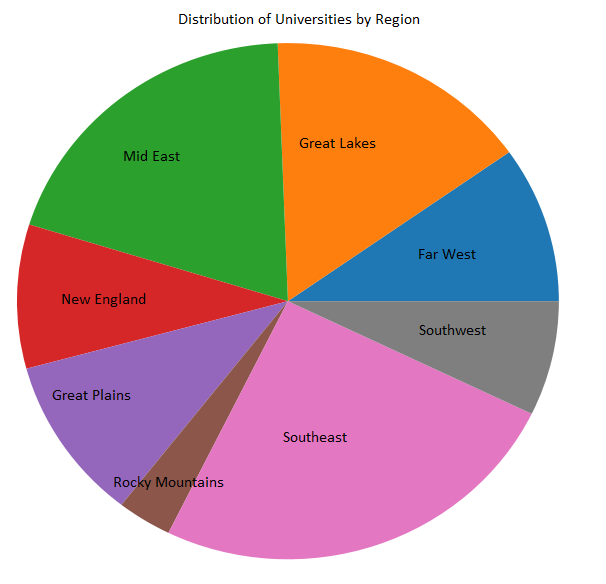
\includegraphics[width = 1.0\textwidth]{Region_Pie_Chart.png}
\FloatBarrier
\section*{5. Scaling}
All of our features (numeric, categorical) required scaling. In general, to keep the weight of each feature the same in the case that the size of the intersect matters, we scaled each feature to 2-3 new binary features. After scaling, we have about 20 features. We list them below:\\
\begin{table}[htbp]
\begin{tabular}{ll}
Public                    & School is public                                                                  \\
Private                   & School is private                                                                 \\
Very Selective Admissions & \textbf{\textless{}} 40\% of students are admitted                                          \\
Selective Admissions      & \textbf{\textless{}} 65\% of students are admitted                                          \\
Regular Admissions        & $\geq$ 65\% of students are admitted                                      \\
New England               & School is in the New England region                                               \\
West Coast                & School is in the Far West region                                                  \\
Inland                    & School is in the Rocky Mountain, Great Lakes, or Great Plains regions             \\
South and Southwest                & School is in the South(east) or Southwest \\
Small Enrollment          & \textbf{\textless{}}1000 undergraduate students enrolled                                 \\
Regular Enrollment        & $\geq$ 1000 undergraduate students enrolled                            \\
Low Aid                   & \textbf{\textless{}} 90\% of students are on financial aid                                  \\
Regular Aid               & $\geq$ 90\% of students are on financial aid                              \\
Low Pell                  & \textbf{\textless{} }30\% of students have Pell Grants                                      \\
Medium Pell               & \textbf{\textless{}} 45\% of students have Pell Grants                                      \\
High Pell                 & $\geq$ 45\% of students have Pell Grants                                  \\
Low Price                 & Average Tuition for Out-of-state students living on campus is \textless{}\$38,000
\end{tabular}
\end{table}
\section*{6. Cross-Validation}
We do a random split of our data 10 times with 30\% being test data and 70\% being training data. We end up with 929 training cases and 399 test cases for each split.
\section*{7. FCA Algorithm}
In general, we translated into code the task prescribed by Fedor Strok and kept the infrastructure as provided with the following changes:\\
We remove unnecessary functions for this task.\\
Because we use different scoring, we remove threshold testing.\\
We report on all of our test files at once.\\
We rewrote infrastructure to track hypotheses.\\
We add our own scoring system.\\
\subsection*{Intersection Scoring}
We have simple intersection scoring and more advanced scoring. If the hypothesis from the intersection is valid (more support than counter-support), then we give one vote to the respective score (positive or negative). This is regardless of the length of the hypothesis or other factors. For advanced scoring, we considered taking the square of the hypothesis (intersect) length and requiring hypotheses to be at least a length of n=4 (or 5,6 etc.) This provides approximately 3\% improvement (77 to 80).
\subsection*{Scoring: Mathematical Notation}
We present the following more rigorous notation for clarification:
Let $h^+,h^-$ be the hypotheses from a intersection of the test case $g^*$ with an example from C+,C-.\\
For a positive hypothesis $h^+$, examples are members of C+ where $h^+$ is a subset of C+ and counterexamples are members of C- where $h^+$ is a subset of C-.\\ 
Next, as we can have an imbalanced amount of positive and negative examples, we need to look at support instead of just the raw number of examples. For a positive hypothesis $h^+$, support is:\\
\begin{equation} 
Support(Positive Hypothesis) = \frac{|h^+ \subseteq C_i+|}{|C+|}
\end{equation}
\begin{equation}
Countersupport(Positive Hypothesis) = \frac{|h^+ \subseteq C_i-|}{|C-|}
\end{equation}
And formally, our scoring is:\\
\begin{equation}
Simple Example Score = 
    \begin{cases}
      1 & support > countersupport\\
      0 & \text{otherwise}
    \end{cases}   
\end{equation}
\begin{align*}
Advanced Example Score = 
    \begin{cases}
      |g^*|^2 & |g^*| \geq n=4, support > countersupport\\
      0 & \text{otherwise}
    \end{cases}    
\end{align*}
\subsection*{Overall Scoring}
For the overall voting, we simply see whether positive or negative scores are higher. We have to divide again by support, otherwise unbalanced data will cause issues.\\
\begin{equation}
Overall Score = \frac{\sum{Positive Example Scores}}{|C+|} - \frac{\sum{Negative Example Scores}}{|C-|}
\end{equation}
\subsection*{A note about maximizing accuracy vs. honesty}
While removing or modifying some of these factors (especially not considering support) will improve the accuracy of this particular data set, it will not make the algorithm useful in general. 
\subsection*{Other Modifications}
We added some timing analysis code, modified code to remove the column headers (the source of 10 'contradictions'), and some other minor things. Lastly, we note that "contradictory" scores from the original code are not contradictions, but rather "unknown" or "unclassifiable". But we only change the end-user display so as to rewrite minimal code. 
\section*{7. Results}
With positive results being that tuition is < \$38,000, and n = minimum hypothesis length:
\begin{table}[htbp]
\begin{tabular}{lllllll}
                                                                                   & Simple   & n $\geq$ 4 & n $\geq$ 6 & n $\geq$ 8 & \textbf{n $\geq$ 12} & n $\geq$ 16 \\
True Positive                                                                      & 1353           & 1432                   & 1432                   & 1459                   & \textbf{1540}                    & 1479                   \\
True Negative                                                                      & 1703           & 1674                   & 1675                   & 1671                   & \textbf{1638}                    & 1561                   \\
False Positive                                                                     & 295            & 324                    & 323                    & 327                    & \textbf{360}                     & 361                    \\
False Negative                                                                     & 629            & 550                    & 550                    & 523                    & \textbf{442}                     & 414                    \\
\textbf{Accuracy}                                                                  & \textbf{0.768} & \textbf{0.780}         & \textbf{0.781}         & \textbf{0.786}         & \textbf{0.798}                   & \textbf{0.797}         \\
\begin{tabular}[c]{@{}l@{}}True Positive Rate\\ (Sensitivity, Recall)\end{tabular} & 0.683          & 0.723                  & 0.723                  & 0.736                  & \textbf{0.777}                   & 0.781                  \\
\begin{tabular}[c]{@{}l@{}}True Negative Rate\\ (Specificity)\end{tabular}         & 0.852          & 0.838                  & 0.838                  & 0.836                  & \textbf{0.820}                   & 0.812                  \\
\begin{tabular}[c]{@{}l@{}}Positive Predictive Value\\ (Precision)\end{tabular}    & 0.821          & 0.815                  & 0.816                  & 0.817                  & \textbf{0.811}                   & 0.804                  \\
Negative Predictive Value                                                          & 0.730          & 0.753                  & 0.753                  & 0.762                  & \textbf{0.788}                   & 0.790                  \\
False Positive Rate                                                                & 0.148          & 0.162                  & 0.162                  & 0.164                  & \textbf{0.180}                   & 0.188                  \\
False Negative Rate                                                                & 0.317          & 0.277                  & 0.277                  & 0.264                  & \textbf{0.223}                   & 0.219                  \\
False Discovery Rate                                                               & 0.179          & 0.185                  & 0.184                  & 0.183                  & \textbf{0.189}                   & 0.196                  \\
F1 Score                                                                           & 0.745          & 0.766                  & 0.766                  & 0.774                  & \textbf{0.793}                            & 0.792                 
\end{tabular}
\end{table}
\subsection*{Results for Tic-tac-toe data}
We are not quite sure what the tic-tac-toe data is for, but we ran our code against it with the following results (TTT $\geq$ n means a minimum hypothesis length was required):\\
\begin{table}[htbp]
\begin{tabular}{llll}
                                         & TTT Simple & TTT $\geq$ 6 & TTT $\geq$ 7 \\
True Positive                            & 477        & 540                  & 613                  \\
True Negative                            & 272        & 328                  & 332                  \\
False Positive                           & 60         & 4                    & 0                    \\
False Negative                           & 149        & 86                   & 13                   \\
Accuracy                                 & 0.782      & 0.906                & \textbf{0.986               } \\
True Positive Rate (Sensitivity, Recall) & 0.762      & 0.863                & 0.979                \\
True Negative Rate (Specificity)         & 0.819      & 0.988                & 1.000                \\
Positive Predictive Value (Precision)    & 0.888      & 0.993                & 1.000                \\
Negative Predictive Value                & 0.646      & 0.792                & 0.962                \\
False Positive Rate                      & 0.181      & 0.012                & 0.000                \\
False Negative Rate                      & 0.238      & 0.137                & 0.021                \\
False Discovery Rate                     & 0.112      & 0.007                & 0.000               
\end{tabular}
\end{table}
\FloatBarrier
(We note that nothing was classified when setting minimum hypothesis length to be $\geq$ 8)
It appears that considering hypothesis of exactly length 7 is extremely useful (we had 98.6\% accuracy). We further note in the appendix that the given code is biased and should only have achieved 66\% accuracy.
\section*{8. Conclusion}
\textbf{We are able to predict with about 80\% accuracy, whether a particular school's tuition will be above or below \$38,000. }\\
While having a minimum hypothesis length improves our accuracy, tuning it seems to give lackluster results. Requiring it to be too high will also cause us to have un-classifiable data. Also, because we chose to split near the median, our accuracy is not as high as possible, but other indicators of predictive value are reasonable. Our predictor is about as accurate as the random forest predictor, so our results are expected.\\
\section*{9. Final Remarks}
\textbf{If we were to improve on this project, we propose the following 3 tasks:}\\
1. Preprocess and process additional features related to student test scores.\\
2. Modify the process to predict a tuition fee rather than do a binary classification task.\\
3. Improve run time with comparison and hypothesis-checking enhancements.

\section*{Appendix}
\subsection*{A final note on 'bias' in the original code}
We believe the original code attempts to do something similar (perhaps with a simpler comparison) to our code. However, we point out that the code has bugs and 'cheats'. We provide code comments as to how this is the case, but also claim the following:\\
The main bug is that we think the variable 't' in 'test\_ impl.py' is some quasi-hypothesis made from the example, but it does not look like a hypothesis but rather a subset of [0,1,'positive','negative'].\\
The main 'cheating' is that this when this 't' contains 'positive' or 'negative', counterexamples will never be found and examples are way more likely to be found.\\
We demonstrate this fact by discarding (removing) 'positive' and 'negative' from t. We cannot think of a scenario where it should be in this set. Rerunning the algorithm gives an approximately 60\% accuracy.
\subsection*{A manual look at Pell data}
Supposing we only used the "Low Pell" split, we would arrive at 69.5\% accuracy:\\
\textit{True Positive = (Low Pell, High Price)}
\begin{table}[htbp]
\begin{tabular}{lll}
           & Low Pell & High Pell \\
High Price & 339      & 319       \\
Low Price  & 86       & 582      
\end{tabular}
\end{table}
\FloatBarrier
\textit{Accuracy = .695, Sensitivity = 0.515, Specificity = 0.871}
\subsection*{A manual look at region data}
\begin{table}[htbp]
\begin{tabular}{llll}
Region          & Low Split & High Split & Predictive Value \\
Far West        & 45        & 78         & 0.634            \\
Great Lakes     & 91        & 110        & 0.547            \\
Mid East        & 94        & 170        & 0.644            \\
New England     & 32        & 93         & 0.744            \\
Plains          & 91        & 48         & 0.655            \\
Rocky Mountains & 23        & 13         & 0.639            \\
Southeast       & 223       & 122        & 0.646            \\
Southwest       & 69        & 24         & 0.742           
\end{tabular}
\end{table}
\textit{One way to interpret this is that given a school is in New England, we would be able to guess with 74.4\% accuracy that tuition costs 38,000 or more}
\subsection*{Sanity Check: Random Forest Classifier}
Using a very naive random forest classifier, we have accuracy of about 80\%, which informs us that our methods are probably reasonable.
\begin{table}[htbp]
\begin{tabular}{ll}
True Positive                            & 1589  \\
True Negative                            & 1578  \\
False Positive                           & 404   \\
False Negative                           & 409   \\
Accuracy                                 & 0.796 \\
True Positive Rate (Sensitivity, Recall) & 0.795 \\
True Negative Rate (Specificity)         & 0.796 \\
Positive Predictive Value (Precision)    & 0.797 \\
Negative Predictive Value                & 0.794 \\
False Positive Rate                      & 0.204 \\
False Negative Rate                      & 0.205 \\
False Discovery Rate                     & 0.203
\end{tabular}
\end{table}
\subsection*{Sanity Check: Excluding 'Useful' Features}
Excluding region and financial aid (Pell, especially) data leads to accuracy rates around 55\%. A quick glance at the data indicates that those are our best indicators. 
\subsection*{A quick reference relating states to regions}
\begin{verbatim}
region_SE = 'Southeast AL AR FL GA KY LA MS NC SC TN VA WV'
region_W = 'Far West AK CA HI NV OR WA'
region_SW = 'Southwest AZ NM OK TX'
region_MNT = 'Rocky Mountains CO ID MT UT WY'
region_NE = 'New England CT ME MA NH RI VT'
region_ME = 'Mid East DE DC MD NJ NY PA'
region_MW = 'Great Lakes IL IN MI OH WI'
region_GP = 'Plains IA KS MN MO NE ND SD'
\end{verbatim}
\subsection*{Run-time Analysis}
Runs are timed with an update every 100 test cases examined. Currently this takes about 15 seconds. A full run presented in the final commit takes approximately 15 minutes.
\end{document}
